\documentclass[11pt]{article}
%Required: You must have these
\usepackage{graphicx}
\usepackage{tabularx}
\usepackage{natbib}
\usepackage{array}
\usepackage{amsmath}
%\usepackage[backend=bibtex]{biblatex}
\setkeys{Gin}{width=0.8\textwidth}
%\setlength{\captionmargin}{30pt}
\setlength{\abovecaptionskip}{10pt}
\setlength{\belowcaptionskip}{10pt}
 \topmargin -1.5cm 
 \oddsidemargin -0.04cm 
 \evensidemargin -0.04cm 
 \textwidth 16.59cm
 \textheight 23.94cm 
 \parskip 7.2pt 
\renewcommand{\baselinestretch}{1.2} 	
\parindent 0pt
\usepackage{lineo}
\linenumbers

\bibliographystyle{..//refs/styles/besjournals.bst}
\usepackage{xr-hyper}
\usepackage{hyperref}


\externaldocument{SUPPperiodicity2021}

\title{Experimental designs for testing the interactive effects of temperature and light in ecology: the problem of periodicity }
\date{}
\author{D.M. Buonaiuto $^{1,2,3,a}$, M. Donahue$^{4}$, E.M. Wolkovich$^{2,3,5}$}

\begin{document}
\section*{Abstract}
\begin{enumerate}
\item Temperature and light cues interact to control many biological processes. Experiments give researchers the ability to manipulate these environmental cues independently, and can be designed to robustly quantify their individual and interactive effects on any particular biological activity. Such experiments have produced important insights into the environmental controls on numerous biological processes in both plant and animal taxa across terrestrial and aquatic environments. Testing the interactive effects of multiple environmental cues, however, requires experimental treatments to be fully independent; any unmeasured experimental covariation among treatments can result in incorrect conclusions.

\item  Using a database of controlled environment experiments on the spring phenology of woody plants as a case study, we highlight how a common experimental set-up, designed to parse the interactive effects of temperature and photoperiod on time to budburst, introduces a latent experimental covariation of these treatments by coupling photo- and thermo- periodicity. Using data simulations, algebraic corrections and a comparative analysis of published experiments, we demonstrate how this unmeasured experimental covariation biases statistical inference regarding the relative contribution of light and temperature cues to phenological variation.

\item We identify this experimental covariation in more than 40\% of published phenology studies that manipulate photoperiod. Our analyses demonstrate that the coupling of thermo- and photo- periodicity results in the overestimation of the effect of photoperiod, the underestimation of forcing effects, and misleading conclusions about their interactions on phenology. This may, in part, explain why the significance of photoperiod cues for spring phenology is currently debated in the literature.

\item Accurate forecasting of how varying environmental conditions will impact the dynamics of biological events requires accurately quantifying cues responses. To this end, we present several alternative experimental designs that can provide more robust estimates of the relative effects of temperature and photoperiod on phenology, and many other biological processes controlled by temperature and light.
%284 words
\end{enumerate}

\textbf{Keywords:}  forcing, full-factorial,  growth chamber, light,  phenology, photoperiod, temperature, thermoperiod \\
\pagebreak
\section*{Introduction}
%Temperature and light dictate numerous biological processes including....\textit{list here}\citep{}. These cues often interact in complex ways, and a major goal of biology is to quantify their both individual and interactive effects on biological activity \citep{}. This effort has only become more critical in recent decades as such measurements are essential for accurately predicting organisms' response to anthropogenic global change and informing biodiversity conservation planning and practices \citep{}.\\
\noindent Across the tree of life, temperature and light availability shape a number of important biological processes including growth and metabolic rates \citep{MacLean:2019aa}, sex determination \citep{Brown:2014vn}, acclimatization to seasonal environments \citep{Hamilton2016} and the timing of life cycle transitions \citep[i.e., phenology,][]{Forrest2010}. These biological responses in turn dictate broad-scale ecological processes and patterns ranging from biogeochemical cycling \citep{Piao2007} to species range limits \citep{Chuine2001}. Characterizing the specific dynamics of how these environmental factors synergistically affect biological processes across a wide range of taxa has become even more important as anthropogenic global change continues to expose organisms to novel environmental conditions \citep{Portner:2008vd}.

%It is difficult to evaluate the individual effects of temperature and light cues and their interactions in \textit{in situ} observational studies because temperature and light variables tend to co-vary in nature \citep{}. However, well designed experiments in controlled environments (e.g. growth chambers, greenhouses, mesocosm) can be used to manipulate temperature and light variables independently, allowing for robust comparisons of their individual and interactive contributions to biological processes. Indeed, this approach has provided many fruitful insights regarding temperature and light signaling over the last century \citep{} and has great potentially to continue to advance fundamental and applied biological inquiries in the decades to come \citep{}.\\
\noindent Because temperature and light availability often co-vary in the field \citep[for example, in most temperate ecosystems, daylength and temperature both increase as the season progresses,][]{Rosenberg1974}, it can be difficult to disentangle their relative contributions to biological processes. In contrast, experimental manipulations of climate variables in artificial environments can mechanistically characterize biological responses to environmental fluctuations \citep{Ettinger:2020aa,Primack2015}. Researchers have used controlled environments of all shapes and sizes to this end \citep{Downs:1980us}; these efforts have greatly advanced our collective understanding of the fundamental biology of a wide variety of organisms and ability to predict ecological and evolutionary responses to current and future climate change \citep{Stewart:2013wz}.

However, controlled environment experiments have their own challenges. Experimentalists must balance biological realism with robust inference, experimental effort with statistical power, and account for the effects of unmanipulated or unmeasured variables \citep{schneiner2001}. Because biological responses to the environment are generally the product of complex interactions between multiple environmental signals \citep{Casal:2002vz}, seemingly small choices about experimental designs can generate significant differences in outcomes. Experimental treatments are rarely standardized among researchers, even within disciplines \citep{Wolkovich_2022}, and these complexities may in part contribute to the many discrepancies between experimental studies and observation data \citep{Poorter:2016aa}. Even with these limitations, controlled environment studies remain a powerful tool to mechanistically assess organismic responses to the environment, provided that the implications of treatment designs are well understood and well matched with the scope of the research question. 

As technology advances and experiments become more complex, researchers can manipulate more variables and multiple axes of variation (e.g., temperature, amplitude, periodicity, wavelength) at the same time. Yet these efforts may present a tradeoff between biological realism and robust inference. Through investigating the literature on experiments with plant phenology, we show that experiments that manipulate both photo- and thermo- periodicity often introduce a latent experimental covariation between light and temperature treatments, which may misrepresent the effects of each of these environmental variables and the interaction between them. We begin by briefly detailing how temperature and light treatments are generally applied in phenology experiments and review the minimum experimental elements required to robustly test interactions between two or more environmental variables. We then detail the problem of inference that can arise when manipulating the periodicity of both temperature and light in experiments, and demonstrate the extent to which this is an issue through data simulations, a mathematical correction, and a comparative analysis of published experiments. Finally, we conclude by outlining several experimental designs that can overcome the problem of periodicity. 

While our case study deals with phenology of temperate woody plants, it provides insights into a number of other systems with parallel issues. Studies of aquatic algae \citep{XU2019167}, insects \citep{ANDUAGA201846}, amphibians \citep{WRIGHT200433} and fish \citep{Olemda_2009} have similarly struggled to disentangle the effects of thermo- and photo- periodicity.  Thus, we believe the potential problems and solutions we present here are broadly applicable to studies on any other organisms and biological processes that utilize temperature and light signals. 

\section*{Case study: Estimating phenological cues from experiments}
Decades of experimental work in controlled environments have demonstrated that temperature (both cool temperatures in fall/winter and warming temperatures in spring) and photoperiod are the primary phenological cues for plants in the temperate/boreal zones \citep{Ettinger:2020aa}. While exposure to cool winter temperatures (chilling) strongly impacts phenology \citep{Laube2014}, we focus here on warm temperature and light treatments, because controlled chilling treatments with light are uncommon \citep{Wolkovich_2022}. Choices about how to apply warm temperature and light treatments, in particular, can compromise inference on their effects, so we focus on these two cues.

While a large variety of experimental designs have been used to study plant phenology, generally experiments tend to manipulate two major axes of light and warm temperature variation:
\begin{enumerate}
\item \underline{Intensity:} The amount or quality of a variable. Here we define temperature intensity as the amount of heat present in the system (measured in degrees). In the phenology literature this measurement is generally referred to as forcing. We define light intensity as the luminosity or irradiance present in the system (measured in lumens or watts). 
\item \underline{Periodicity:} The interval at which the intensity of the variable is applied. Hereafter, we refer to the periodicity of light as photoperiod (often used synonomously with ``daylength") and the periodicity of temperature as thermoperiod. 
\end{enumerate}
For phenology, photoperiodicity is generally considered the primary light cue for plants \citep{WAY:2015aa}, \citep[though regarding light intensity and phenology see][]{Brelsford2018,Cober1996}. For temperature, conventionally both intensity and periodicity drive phenological activity and several metrics (e.g. growing degree hours, thermal sums, growing degree days)  that combine these two axes have been developed \citep{Gu:2016wa}. The importance of thermo-intensity and periodicity is well supported; under natural conditions diurnal temperature fluctuations in temperate regions can be quite large in the spring, and studies have found that diurnal temperature variation strongly influences plant phenology \citep{Burghardt:2016uy}. In fact, even if thermoperiodicity is not an explicit treatment variable (i.e., manipulated systematically), incorporating it in experiments can be essential for translating experimental results into real world predictions \citep{plants9101312}.

Like many other biological processes, recent advances have demonstrated that plant phenological responses are nonlinear, due largely to interactions between cues \citep{Wolkovich_2022,fu2015}, highlighting the need for experiments designed to evaluate the strength of these interactions. To have the statistical power to partition the individual and interactive effects of two or more variables, an experiment must:
\begin{enumerate}
\item Have at minimum of two treatment levels of at least two variables.
\item Treatment levels must be full factorial (Fig. \ref{fig:examp}a.). Full factorial designs are both balanced (Fig. \ref{fig:examp}b.)  and orthogonal (Fig. \ref{fig:examp}c.); meaning that all possible treatment combinations are applied and each treatment is independent of all others \citep{cheng2016}.
\end{enumerate}

These two critical elements may seem obvious but are conspicuously absent from many published studies.  Using a recently published database of woody plant phenological experiments, OSPREE: Observed Spring Phenological Responses in Experimental Environments \citep{wolkovich2019}, we found that out of 152 controlled environment experiments (across 93 studies) only 18 manipulated both light and forcing cues with a design that was both balanced and orthogonal. But even experiments that are designed to be full factorial frequently violate the assumption of orthogonality when both photo- and thermo- periodicity are built into experiments. We detail this problem below.
% old. This notable dearth of robust tests of light and temperature interactions may stem from the common limitations of time, space, and resources that experimentalists often face, but it may equally relate to a fundamental issues that arises from the fact that these variables themselves are comprised of multiple axes of variably.\\
%\section{Axes of environmental variation in experiments and their implications}

\section*{The problem of periodicity}
A common approach in phenology experiments that seems to balance prior knowledge about the underlying physiology of phenology, biological realism and experimental inference is to vary photoperiodicity, and thermal intensity and periodicity \citep[e.g.,][]{Flynn2018,Sanz-Perez:2009aa,Basler:2014aa}. For example, a basic experiment might include a long (16 hours) and short (8 hours) photoperiod treatment and a high (25/15$^{\circ}$C day/night) and low (20/10$^{\circ}$C day/night) forcing treatment. In this case, the thermoperiodicity is not an explicit treatment (both high and low temperature treatments use a diurnal fluctuation of 10 $^{\circ}$C), and is simply incorporated in the design to enhance biological realism. At first glance, this design appears to meet the criteria of a full factorial design, multiple treatment levels that are balanced and orthogonal, with high/low temperature treatments (mean 20$^{\circ}$C and 15$^{\circ}$C respectively) and long/short photoperiod treatments applied in all possible combinations.

Yet the orthogonality of this design is based on the assumption of a 12 hour thermoperiod. If, rather the thermoperiod is coupled with the photoperiod, the temperature treatment is non-orthogonal because the daily mean temperature of the long/high treatment will be higher than that of the short/high treatment, and the long/low treatment slightly warmer than the short/low. We refer to this experimental set-up as a coupled design (i.e. thermoperiod and photoperiod are coupled with each other).  %(Fig \ref{fig:ortho}a). %could also phase this in growing gregrees
Coupled designs introduce an experimental covariation between photoperiod and forcing treatments. This experimental covariation is clearly illustrated when temperature treatment levels are converted to thermals sums. We calculate thermal sums (also called growing degree hours), by multiplying hourly temperatures above a certain base temperature threshold by the number of hours for which they are applied over a 24 hour period \citep{Parent:2019ug}. For example, given a base temperature of 0$^{\circ}$C, a low forcing treatment of 20/10$^{\circ}$C day/night accrues 400 thermal units per 24 hours  when crossed with the long (16 hour) photoperiod treatment and only 320 thermal units when crossed with the short (8 hour) photoperiod treatment. While this experimental covariation among the photoperiod and temperature treatments is biologically realistic, it makes it statistically impossible to differentiate the independent and interactive effects of temperature and photoperiod on any given biological process.

This problem of inference that arises from the experimental covariation of thermo- and photo- periodicity is not limited only to studies seeking to directly compare the effects of photoperiod and forcing; it applies in any study evaluating the influence of photoperiod on biological activity, even if it is the only manipulated cue. Experimentally isolating the effect of photoperiod assumes that all other environmental variables are held constant.  Similar to the case described above, % for comparing the interactive effects of photoperiod and forcing, 
the coupling of photoperiod and thermoperiod in an experiment where forcing is supposed to be a consistent, background condition (e.g., two levels of photoperiod treatments of 8 and 16 hours, both at a background temperature of 20/10$^{\circ}$C day/night) would yield a situation in which longer photoperiod treatments were also receiving more---unmeasured---heating than shorter photoperiod treatments. In this case, some amount of the perceived photoperiod effect is due to the latent, increased forcing, and the experiment will not isolate the true effect of photoperiod.

We queried the OSPREE database to identify experiments that applied different day and night temperatures in their studies without designating diurnal temperature variation as an explicit experimental treatment. Of the 51 experiments in the OSPREE database that manipulated photoperiod experimentally, up to 43\% of them appear to include an experimental covariation with thermoperiod. Of the 18 studies that manipulated both photoperiod and temperature interactively, we found that up to 55\% of them appear to have this issue, suggesting that the true interactive effects of these cues on spring phenology is quite poorly characterized. This may be in part why the relative contribution of temperature and photoperiod cues to spring phenology remains a contentious debate in the phenology literature \citep{koerner2010a,CHUINE:2010wg,Jennifer:2010un}.

\section*{Periodicity and inference}
%EMW17Jun2022: possible to cut 'on spring phenology ' in sentence below?
If the lack of orthogonality introduced to experiments when photoperiod and thermoperiod are coupled is overlooked, regression models will always overestimate the photoperiod effect and underestimate the forcing effect (Fig. \ref{fig:3d}a,b.). This is because forcing is the variable with latent, unmeasured variation. In the case of phenology, this is particularly significant because studies repeatedly suggest that forcing is a more dominant cue than photoperiod for spring phenology \citep{CHUINE:2010wg,Zohner:2016uz,Gauzere2019}.

If experiments are designed to quantify the interaction between photoperiod and forcing, here too, the experimental covariation of periodicity will result in an erroneous estimation of the interaction. (Fig. \ref{fig:3d}c,d.). Our simulation depicts a particularly troublesome case where a true sub-additive interaction is interpreted as a supra-additive one (Fig. \ref{fig:3d}c,d.), however, other outcomes are possible. Experimental covariation of light and temperature treatments due to coupling thermo- and photo- periodicity will generally result in the incorrect estimation of the interaction term, but the exact nature of this statistical issue depends on the sign and strength of the interaction.
%, therefore we should \emph{a priori} expect the covariation between photo- and thermo-period may result in an over-estimation of the photoperiod effect. %and a weaker estimate of the interaction between photoperiod and forcing. DB I checked this and we still underestimate photoperiod even when it is a stronger effect
%
%old parapgraph\textbf{We can mathematically solve for how much of an estimated photoperiod effect is due to forcing---in experiments where they covary---by making several major asssumptions. If we assume forcing and photoperiod effects are additive, linear and there is no interaction between the two effects, then we can solve (algebraically) for the estimated effect of forcing and photoperiod given an orthogonal treatment design (see Fig. \ref{fig:3d}, Supporting info). Using estimates from one experiment that covaried forcing and photoperiod effects \citet{Flynn2018}, we found roughly two-thirds of the estimated photoperiod cue could be due to forcing effects.} % Lizzie says -- estimated effect of 4.5 in the paper, while in the supp we show 3 could be due to co-variation. 

We can attempt to estimate how much of a photoperiod effect is due to forcing in experiments where they covary by making several major assumptions. Our major assumptions are that forcing and photoperiod effects are additive and linear (i.e., there is no interaction). While this may not be true in nature, it gives us insight into the potential effect of the experimental covariation of periodicity by allowing us to solve algebraically for the separate effects of forcing and photoperiod. We replace the qualitative factor (high/low forcing) by the quantitative effect of forcing (thermal sums) to properly account for the difference in forcing between short and long photoperiods (see Supporting Information: Estimating the effects of experimental periodicity covariance mathematically). Using the data from one experiment that experimentally coupled thermo- and photo-period, \citet{Flynn2018}, we found that 33\% of the published photoperiod effect of 4.5 days could be due to forcing. 

Our algebraic solution cannot be as readily applied in experiments that assume photoperiod and forcing interact. However, we can generally assess the scope of the problem of inference due to experimental covariation of periodicity by comparing studies that used a coupled design to those with alternative approaches. While we are aware of no experiments that explicitly compare the effects of experimentally coupling vs. uncoupling photo- and thermo- periods, we identified two phenology experiments that utilized many overlapping treatment levels and species from the same sampling sites, however in one study, \citet{Flynn2018}, photo- and thermo- period experimentally co-vary, while in the other, \citet{Buonaiuto:2021ug},  photo- and thermo- period were varied independently. Comparing the cue estimates from these two studies offers an opportunity to test our theoretical and mathematical predictions, and further understand the uncertainty in cue estimates due to coupled periodicities.

We subset each dataset to include only the species shared among the two studies, and re-analyzed the data using Bayesian hierarchical models to compare the difference in the photoperiod, forcing and interaction estimates (see Supporting Information: Modeling Methods). We found that the estimated differences in the mean response to photoperiod and forcing and their interactions among study designs were on the same order as our predictions above for misestimated cue effects due to experimental covariation between light and temperature treatments. We estimated a substantially weaker (less negative) photoperiod effect, and marginally stronger forcing effect for the uncoupled vs. coupled experimental design (Fig. \ref{fig:compy}). The interaction term we estimated for the uncoupled design was negative, suggesting the interaction between photoperiod and forcing is supra-additive, while the estimated interactive effect from the coupled design was sub-additive (Fig. \ref{fig:compy}).

Unlike in our simulations (Fig. \ref{fig:3d}), in this comparison we cannot assess what the ``true" effects of these variables are. There are almost certainly other factors driving the differences between these experiments. Both were conducted in different years, sampled different individuals from the population, and used different methods for applying chilling pre-treatments \citep{Flynn2018,Buonaiuto:2021ug}. However, because this comparison is well matched to our predictions and prior knowledge about how temperature and photoperiod are expected to interacting in phenology, we argue that the influence of experimental covariation on statistical inference is apparent enough to take seriously.\\

\section*{Paths Forward}
We have demonstrated that experiments that coupled thermoperiod and photoperiod cannot robustly differentiate the individual or interactive effects of temperature and photoperiod on spring phenology (or any other biological process) due to an unmeasured experimental covariation among temperature and light treatments. Given the paucity of interactive studies in the literature, it is clear that we need more well designed studies to better characterize the effects of these cues. Below we offer several generalized experimental designs that improve statistical orthogonality of controlled environment experiments, which could be further developed and adjusted to fit the needs of experimentalists across many sub-fields of ecology and evolutionary biology. 
\begin{enumerate}
%\item \text bf{Experimental covariation photo- thermo- period with quantified uncertainty}. It may be that the experimental design that best balances environmental realism, statistical inferences and translatability to observational studies are designs that couple periodicity to mimic natural systems (\ref{fig:ortho}a.). Moving forward, researchers using this design need to be aware of the non-orthogonality of this design, and be sure to present the uncertainty surrounding their cue effect estimates, which could be done using a similar mathematical approach to the one we present in this paper (see Supporting Information).
\item \textbf{Manipulate photoperiod and temperature intesity with no thermoperiodicity}. The simplest  way to evaluate the individual and combined effects of temperature and photoperiod in experimental settings is to remove thermoperiodicity from studies entirely by maintaining constant day/night temperatures within temperature treatments (Fig. \ref{fig:designs}a.). This approach allows for the maintenance of statistical orthogonality across treatment combinations. The main drawback is that this design sacrifices the biological realism of diurnal temperature variation, which may make it more difficult to translate estimates from experiments to real-world applications.

\item \textbf{Uncouple thermoperiod and photoperiod}. By varying thermoperiod and photoperiod independently, statistical orthogonality can be maintained across treatments. For example, a study could apply photoperiod treatment levels of 8 vs. 16 hour day/night with a 12 hour thermoperiod regime across temperature treatments (Fig. \ref{fig:designs}b.). While this approach allows for more robust evaluation of cue effects and interactions, uncoupling photoperiod and thermoperiod can require newer and more expensive technologies which many not be widely available. Further, this approach may also introduce new artifacts that occur from the biological rather than statistical interactions between light and temperature \citep{Chew:2012wj}. There is evidence that increasing temperatures in the first two hours of daylight can be almost as effective for stimulating shoot elongation as similar temperature increases for the whole photoperiod \citep{Erwin1998}. With this design, treatments must inherently differ in the amount of time the warmer daytime temperature extends into the dark, nighttime light regime (or vice versa), introducing a new axis of non-orthogonality. %EMW17Jun2022 should it read: 

\item \textbf{Include thermoperiodicity as an explicit experimental treatment}. In many study systems in which both photoperiod and thermoperiod influence biological processes, experimentalists often include thermoperiodicity as an explicit experimental treatment with both constant and varying day/night temperatures applied as separate treatment levels \citep[e.g.,][]{Zaslavksi_1995}. Such experiments would be well suited to compare the relative strength of temperature and light cues and their interactions, and could also assess the relative importance of temperature intensity and periodicity (Fig. \ref{fig:designs}c.). While this study design would offer the promise of robust inference on the importance of interactive environmental cues, executing such an experiment with a full-factorial design would substantially increase the size of a study and its experimental effort. 
\end{enumerate}

In correcting one problem, each of these designs introduces another, which may in fact be an intrinsic property of any experimental manipulation. It may also be that the experimental design that best balances environmental realism, statistical inference and translatability to observational studies are designs that continue to couple periodicity to mimic natural systems. Moving forward, researchers using this design need to be aware of its non-orthogonality, and carefully consider how to present the uncertainty around their effect estimates. It would be useful for researchers to explicitly test how cue estimates vary among experimental designs, and which design is most useful for predicting biological responses to environmental cues in the field under current and future climate conditions. In the meantime, we hope that this issue is a reminder that, as experimentalists, we must continue to be thoughtful about matching our experimental designs to the goals of a study, and be transparent about uncertainty around our experimental inference.

\bibliography{..///refs/periodicity.bib}

\begin{figure}[h!]
    \centering
 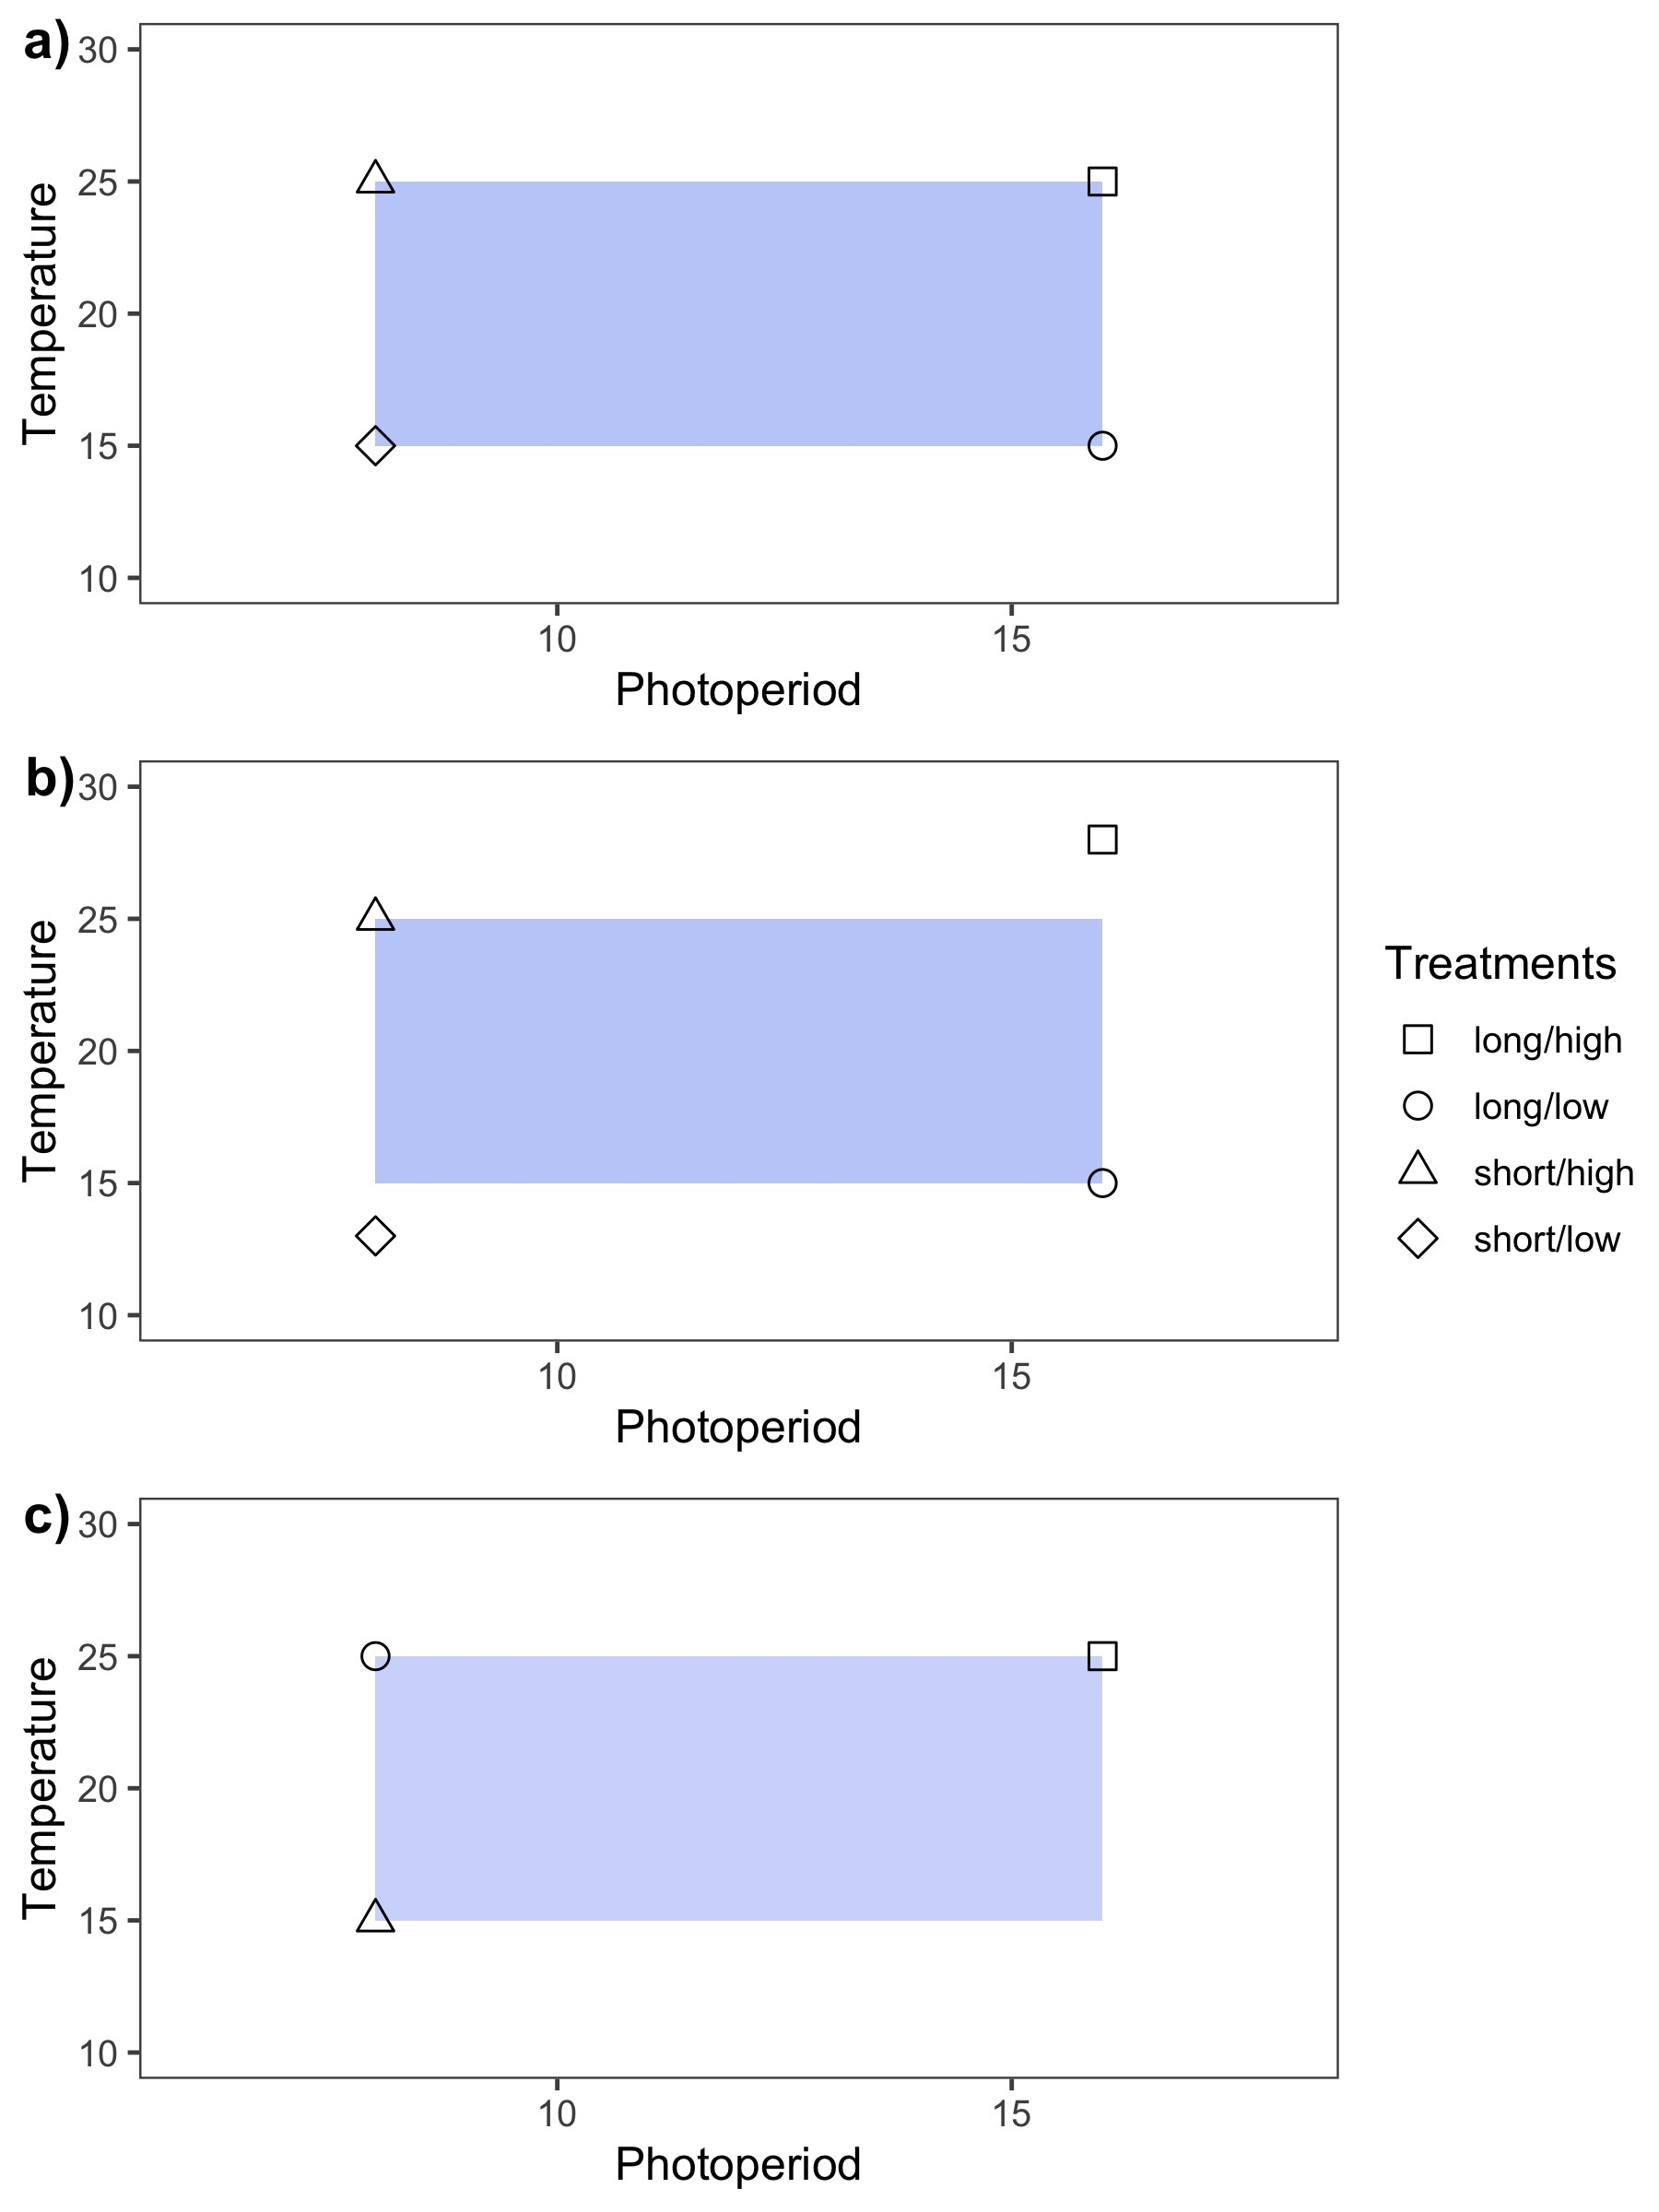
\includegraphics[width=.8\textwidth]{..//Plots/periodicity_figures/factorial.jpeg}
    \caption{Idealized experimental designs demonstrate three approaches for varying temperature and light treatment levels in controlled environment experiments. Design \textbf{a)} is full factorial in that treatments levels are balanced and orthogonal. This design is appropriate for testing interactions between two (or more) variables. In \textbf{b)} the design is balanced but not orthogonal. Non-orthogonality in experiments can arise when experimental covariation among the manipulated variables is not accounted for. In \textbf{c)}, the experimental design is orthogonal but unbalanced. Lack of balance in experiments often arises due to time, space or resource limitations. }
    \label{fig:examp}
\end{figure}

 \begin{figure}[h!]
    \centering
 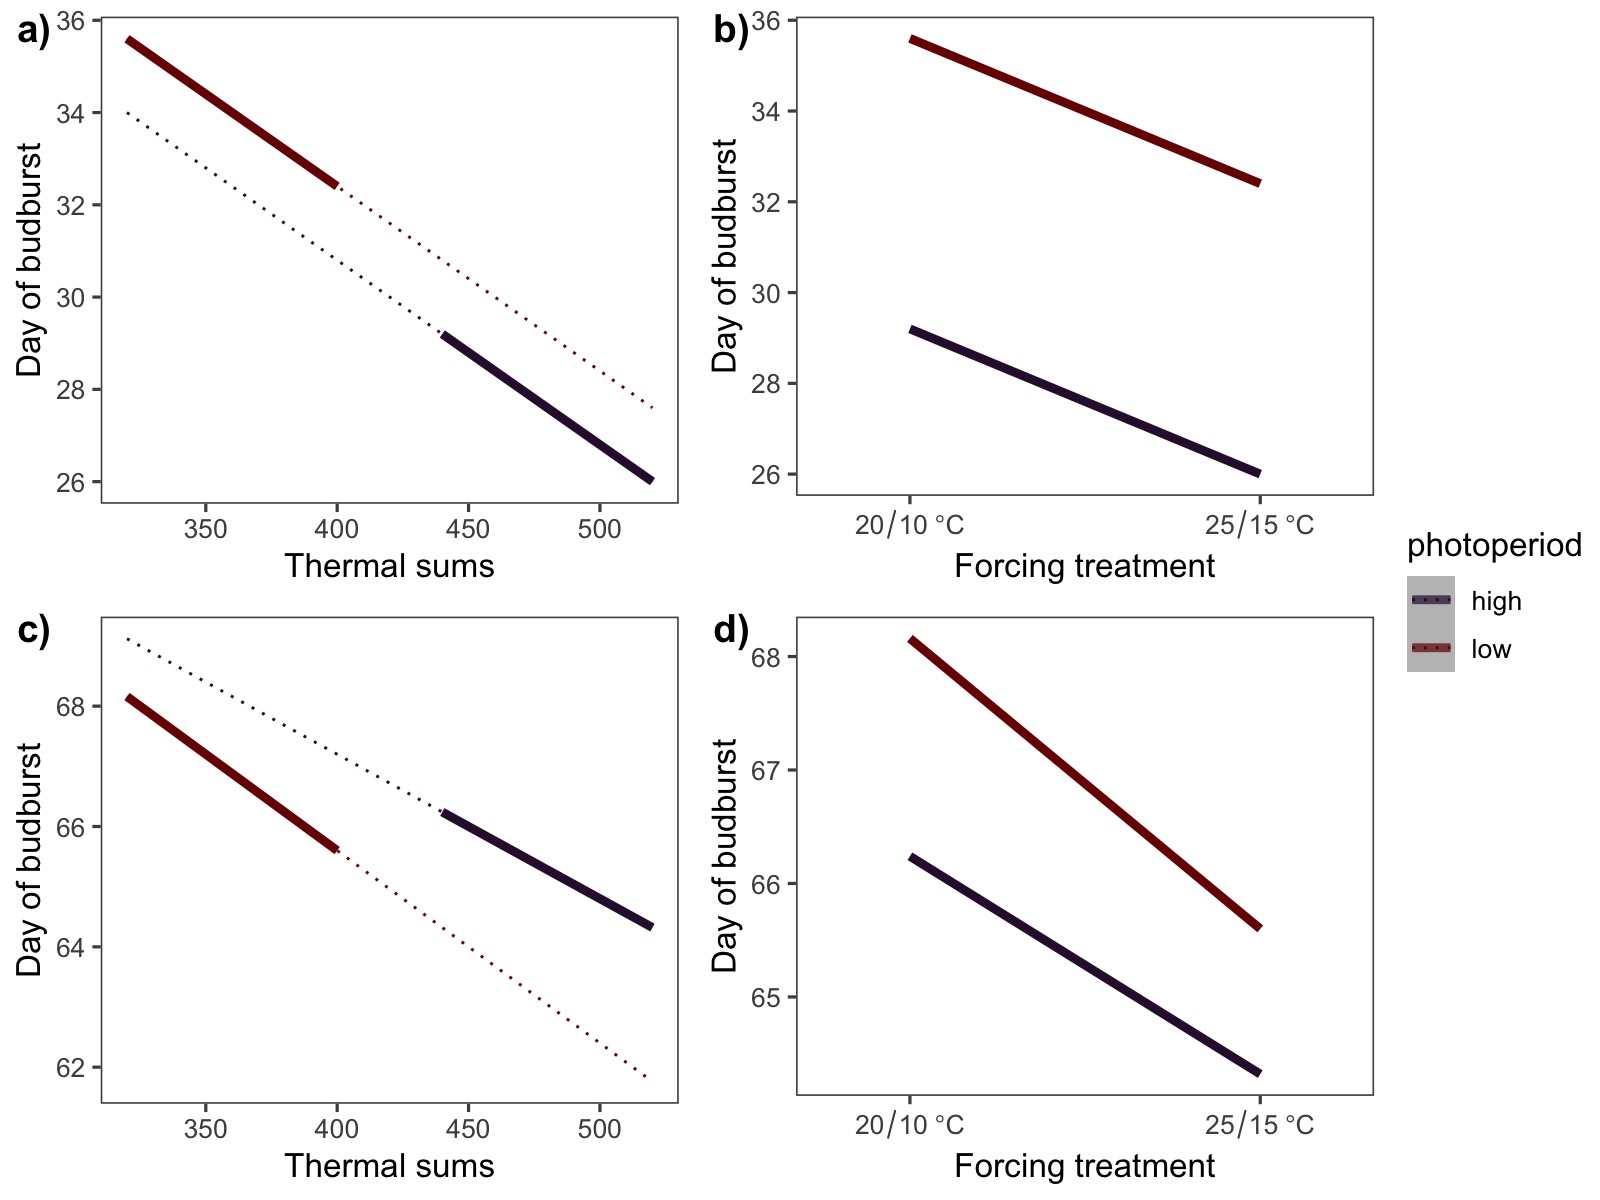
\includegraphics[width=.8\textwidth]{..//Plots/periodicity_figures/apparent.jpeg}
    \caption{Estimated effects of photoperiod and forcing on spring phenology based on a simulated experiment in which the coupling of photoperiod and thermoperiod introduce an experimental covariation between the temperature and light treatments. The dotted lines in \textbf{a)} and \textbf{c)} depict the true effects of forcing at each photoperiod level, and the solid lines depict the estimated effects. \textbf{a)} depicts a scenario where forcing and photoperiod effects do not interact, while \textbf{c)} includes an interactive effect. \textbf{b)} and \textbf{d)} depict the estimated effects of forcing and photoperiod if the experimental covariation due to periodicity coupling in \textbf{a)} and \textbf{c)}, respectively, is unacknowledged.}
    \label{fig:3d}
\end{figure}
 
\begin{figure}[h!]
    \centering
 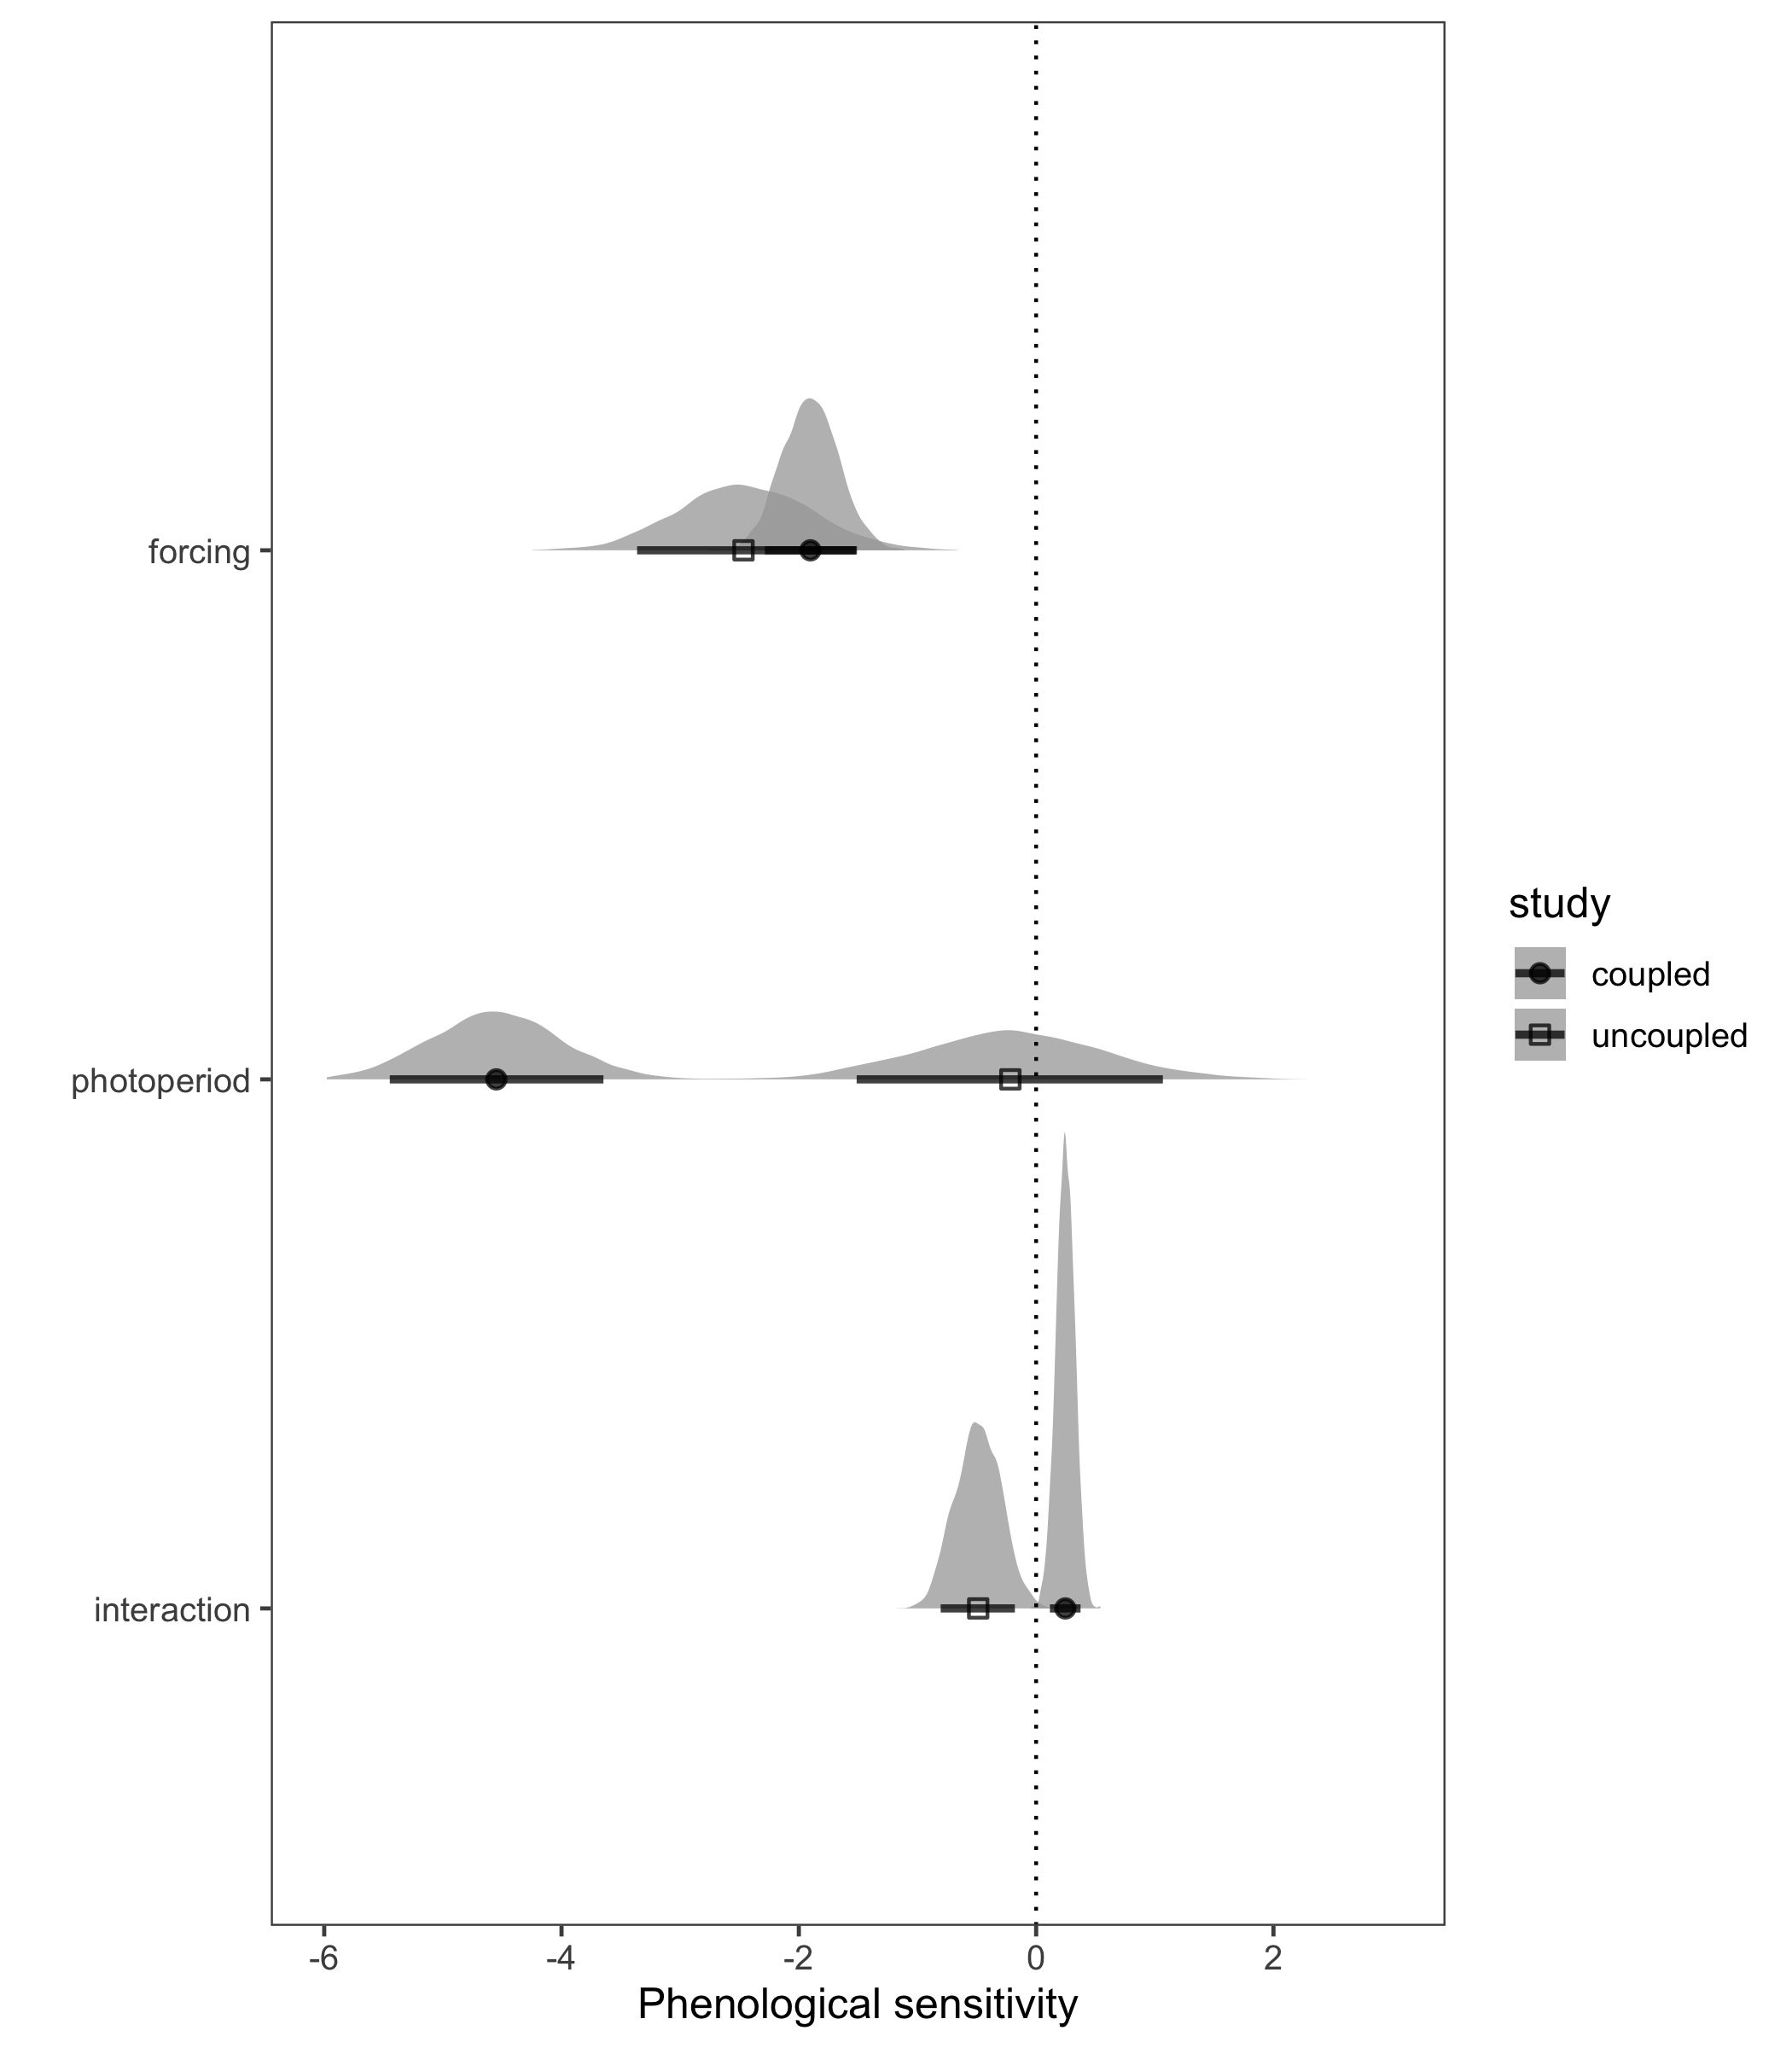
\includegraphics[width=.8\textwidth]{..//Plots/periodicity_figures/modelcomps_winter.jpeg}
    \caption{Estimated phenological sensitivity ($\Delta$ day of leaf expansion/$\Delta$ unit increase in cue level), using alternative methods of varying thermoperiod relative to photoperiod. Points indicate the estimated mean effect and bars the 90\% uncertainty intervals. The full posterior distributions for each parameter are also depicted as an additional display of uncertainty. The coupled thermo- photo- period design is from \citet{Flynn2018} and the uncoupled design is from \cite{Buonaiuto:2021ug}.}
    \label{fig:compy}
\end{figure}

\begin{figure}[h!]
    \centering
 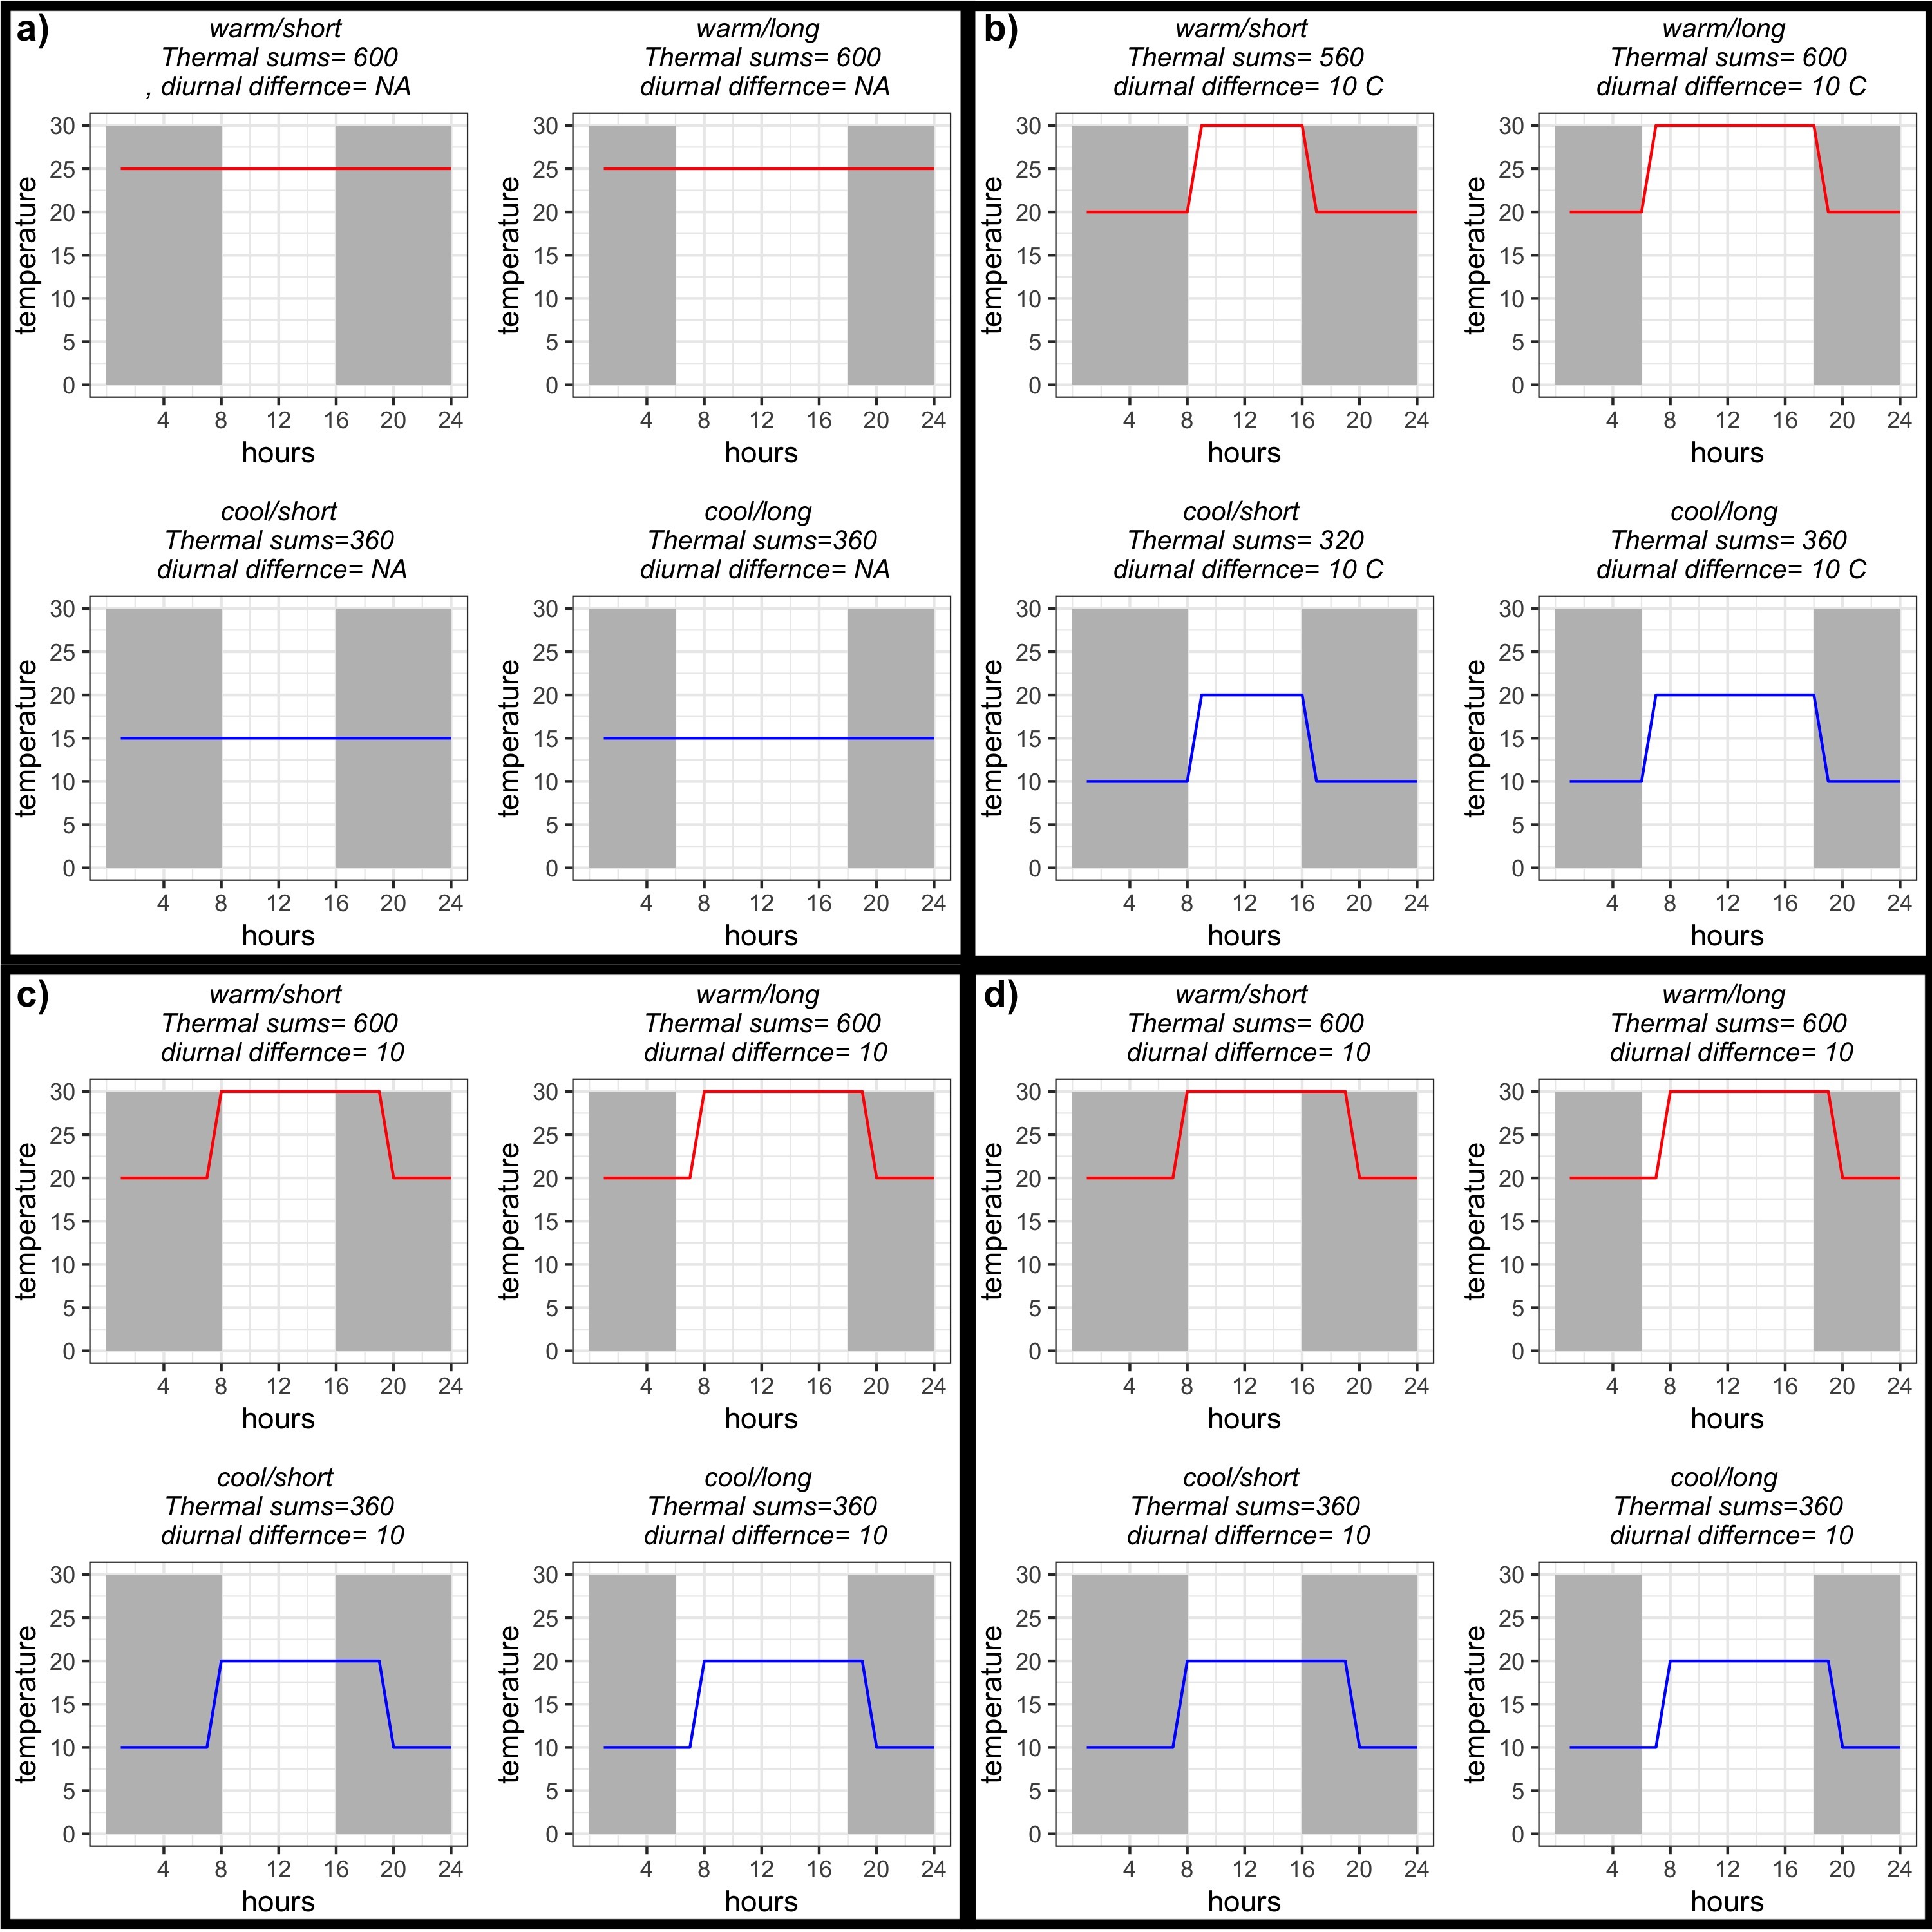
\includegraphics[width=\textwidth]{..//Plots/periodicity_figures/designs.jpeg}
    \caption{Conceptualized experimental designs to test temperature and daylength interactions on a biological response. Design \textbf{a)}  manipulates temperature intensity only (no thermoperiodicity). In design \textbf{b)}, consistent diurnal temperature fluctuations are maintained but, thermoperiod and photoperiod are decoupled and varied independently, maintaining orthogonality in daily temperature treatments. In \textbf{c)}, thermoperiod is included as an explicit experimental treatments to evaluate the individual and interactive effect of photoperiod, temperature and thermoperiodicity.}
    \label{fig:designs}
\end{figure}
 

\end{document}




\begin{enumerate}
\item Temperature and light control and signal many biological processes.
\item They often interact, substitute or compensate for each other.
\item A major goal of biology is to quantify their effects and interactions
\item This has become extra important for predicting organism's response to global change
\item This task cannot be done well through observational studies as light and temperature regimes usually co-vary
\item Experiments in controlled environments (growth chambers, greenhouses etc) can do this, using experimental treatment to partition the effects of this variables and their interactions.
\item Indeed much progress has been made with this approach
\item But experiments must balance many competing factors in their designs, biological realism with statistical inference, the effect of unmeasured climate variable, blocking effects etc.
\item In the sections below we highlight a particular problem that can arise when designing experiments to partition the effects of temperature and daylength and understand their interaction. Our example uses woody plant phenology as an example, but the approach we detail here is relevant for other organisms and biological process too.  
\end{enumerate}

\section{Phenological response to Temperature and Light}
Here a very brief (one paragraph) overview of how light and temperature influence spring phenology. Keep it basic (Warming accelerate phenology, photoperiod might be a threshold), acknowledge chilling is important too, but our example won't really focus on it. Leave some open questions about their interactive nature.

\section{Testing Interactions}
\begin{enumerate}
\item To test interactions and partition effects among two variables that co-vary in nature one must:
\item Have at least 2 treatment levels of each variable of interest
\item Apply them orthoginality, factorially (\ref{fig:examp}, blue box) and define these terms.
\item This may seem obvious but is rarely done. In the case of phenology, a recent analysis of controlled enviroonment study found that only X of Y studies manipulated both light and temperature cues in the same experience and only Z of X did so orthoginally.
\end{enumerate}
\section{Axes of environmental variation annd their there problem}
\begin{enumerate}
\item A further complication arises when decided how to apply each treatment.
\item For any environmental variable there are two axes of variation that can be manipulated in an experiment.  
\item Intensity: Temperature, luminosity. 
\item Period: Thermoperid, Photoperiod.
\item There are measures that incorperate both period intensity (ie growing degree hours).
\item For light cues, photoperiod is the primary phenolgoical cure
\item For temperature, period and intesity matter. For example, temperture in nature varies diurnally and dirunal temperature fluctions may contribute to the phenology signal, or at the very least, lack of them might make phenology wonky. 
\item Therefore a common approach in experiments that seems to balance prior knowlege, biological realism and experimental inferences is to vary photo period, and temperature intensity and period. 
\item Clarify with an example. 12 and 8 hours of daylength. 30/20 and  20/10 temperature (or whatever I said in the figure).
\item If not carefully handled this approach can introduce a nonorthogicanity into the experiment, biasing inference.
\item If the thermo-periodicity and photoperiodcity are coupled (ie the night time temperatures begin when the lights go off, and the day time temperatures begin when they turn back on) The impact is that that the high temperautre high/long photoperod treatment more cumulative heat than the high temperature/short photoperiod treatment throughout the experiment as can be seem when the temperature treatment are converted to thermal sums (\ref{fig:examp},(\ref{fig:ortho}b)). To state this more simply, though the applied temperatures are the same sicne their are applied for different durations, the mean daily temperature differ among the temperature treatments.
\item This non-orthoginality makes it stasticially impossible to differentiate the effect of the photoperiod and temperature treatments.
\end{enumerate}
\section{Quantifying uncertainty}
\begin{enumerate}
\item To estimate the extent to which this non-orthangonical could bias results we intergated the results from a large scale experiment that included a coupled thermo-photoperid design. We used plane geometry to estimate how much of the estimated forcing effect (the assumed dominant cue) may actually be attributed to change in photoperiod. The calcualtions can be found in the suppliment.
\item While the original model estimates of the forcing and photoperiod effects (phenological sensitivy; $\Delta$ phenological event day/ $\Delta$ cue level) were estimate 9.5 and 4.5 advance we estimate that as much about 3.0 (units?) of the forcing effect could be attributed to the photoperiod effect.
\item It is important to stress that this is not a model correction. The original model could acutally before correct or it could in fact have understimated the true forcing effect and infalted the photoperiod effect. We simply cannot say this. (\textit{Probably should think about how to phase all this without making it seem like the Flynn paper is wrong}).
\item Our estimate of ``how much of the reported photo-period response could in actuality be driven by the latent differences in thermo-period" can be rephrased as a prediction of the expected difference in estimated photoperiod sensitivity between a coupled and decoupled photo- and thermo-period experiment.
\item While we are aware of no experiments that explicitly test these different designs, a phenological study by \citet{Buonaiuto:2021ug} applied serveral treatments levels that overlap with those in the \citet{Flynn2018} study to twig cuttings from the same source population. However in the second study the authors decoupled photo- and thermo-period. After subseting each dataset to  include nly species and treatment levels common amoung them, we re-analyzed the data (see supplimental method) and found that difference in the average response to photoperiod amoung study designs  was on the same order our mathmatical prediction see figure, though the photoperiod effect was in fact weaker in the uncoupled dataset (\ref{tab:compy}).\\
\item  With such significant uncertainty in partitioning the effect of forcing and photoperod even in experiment, this might contribute to the debate about the importance of photoperiod.
\item Below we outline several solutions to this experimental design, that should inprove the inference from growth chamber studies
\end{enumerate}

\section{Solutions}
\begin{enumerate}
\item Manipulate temperature intesity only and photoperiod. You estimate interactions because you have multiple levels of temperature and orthogiality. Lose some biological realism (\ref{fig:ortho}a).


\item Uncouple thermoperiod and photoperiod. As done in \citet{Buonaiuto:2021ug}. While this is probably better than coupled approach as it account for statistical interaction, it may introduce new artifact that occur from biological interactions. For example evidence from horticulture studies have demonstrated that cell growth is most sensitive to temperature fluctuation at the beginning of the photoperiod\citep{Erwin1998}. \citet{Erwin1998} found that increasing temperatures in the first two hours of the photoperiod was almost as effective for stimulating shoot elongation as similar temperature increases for the whole photoperiod (\ref{fig:ortho}c).

\item Set temperature treatments using metrics that account for period and intestist. Growing degree hours.maintain mean temperature and set photoperiod legnths and thus thermal orthoginality in expiriment by proportionately varying diurnal fluctionation accross treatment level. However, if the differenes between day and night temperature has a meanful biological effect as has been shown, this introduces another confonding, non-orthoginal factor (\ref{fig:ortho}d).

\item While this improvements should improve our ability to assess light and temperature interactions in biology, their challenges should aslo remind us to be humble with inference and think critically about what is, and isn't accounted for.
\end{enumerate}

%EMW20Feb22: I feel like the chilling details are not critical ... see what you think of above edits 
% CUT: are usually applied in a pre-treatment either by sequentially removing plant materials from the field throughout the winter dormancy period \citep{limitingcues} or applying experimental chilling in a cold chamber before warm temperature and light treatments are applied in tandem \citep{Weinberger:1950aa,Flynn2018
